\begin{figure}[h]
\centering

%-------------------------------%
% Left image: 2D Overlap
%-------------------------------%
\begin{minipage}{0.48\linewidth}
\centering
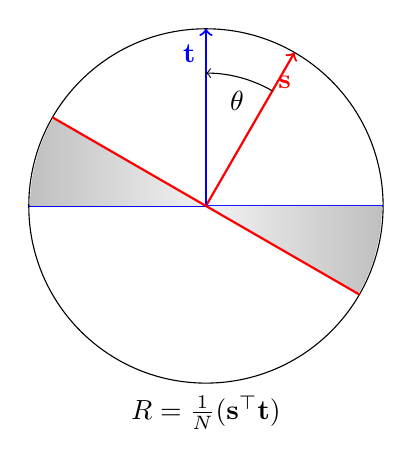
\begin{tikzpicture}[scale=1.5]

    % Circle
    \draw (0, 0) circle (1.5cm);

    % Vectors s (red at 60°) and t (blue at 90°)
    \draw[->,thick,red]  (0,0) -- (60:1.5cm) node[pos=0.7, above right] {\(\mathbf{s}\)};
    \draw[->,thick,blue] (0,0) -- (90:1.5cm) node[pos=0.75, above left] {\(\mathbf{t}\)};

    % Angle theta (between s & t)
    \draw[<-] (0,1.125) arc (90:60:1.125cm) node[pos=0.7, below left] {\(\theta\)};

    % Blue lines (perp. to t = 90°)
    \draw[thick,blue] (0,0) -- (-1.5,0);
    \draw[thick,blue] (0,0) -- ( 1.5,0);

    % Gray shading for overlap region
    \shade[left color=gray!50, right color=gray!10]
      (0,0) -- (-1.49,0) arc (180:150:1.5cm) -- cycle;
    \shade[left color=gray!10, right color=gray!50]
      (0,0) -- (1.49,0) arc (0:-30:1.5cm) -- cycle;

    % Red line(s) perp. to s (60°)
    \draw[thick,red]  (0,0) -- (150:1.5);
    \draw[thick,red]  (0,0) -- (330:1.5); % same as -30°

    % Overlap formula
    \node at (0,-1.75) {\( R = \frac{1}{N} (\mathbf{s}^\top \mathbf{t}) \)};

\end{tikzpicture}
\end{minipage}%
\hfill
%-------------------------------%
% Right image: 3D Overlap (conic sections + wedge)
%-------------------------------%
\begin{minipage}{0.48\linewidth}
\centering
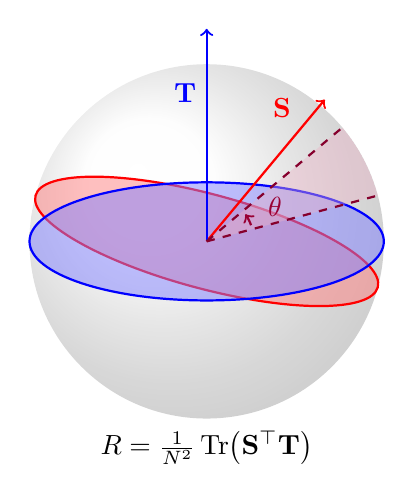
\begin{tikzpicture}[scale=1.5]

    % Light-gray "sphere"
    \shade[ball color=gray!5, opacity=0.3] (0,0) circle (1.5cm);

    % --- Red ellipse for S (unchanged) ---
    \begin{scope}
      \clip (0,0) circle (1.5cm);
      \fill[red!50, opacity=0.5]
        [rotate around={-15:(0,0)}, xscale=1.5, yscale=0.4]
        (0,0) circle (1.0);
    \end{scope}
    \draw[thick, red]
      [rotate around={-15:(0,0)}, xscale=1.5, yscale=0.4]
      (0,0) circle (1.0);

    % --- Blue ellipse for T (CHANGED) ---
    % Make it near-horizontal (rotate=0 or a small angle),
    % and bigger horizontally by increasing xscale significantly.
    \begin{scope}
      \clip (0,0) circle (1.5cm);
      \fill[blue!50, opacity=0.5]
        [rotate around={0:(0,0)},    % CHANGED: no tilt so near x-axis
         xscale=1.5, yscale=0.5]     % CHANGED: bigger horizontally
        (0,0) circle (1.0);
    \end{scope}
    \draw[thick, blue]
      [rotate around={0:(0,0)}, xscale=1.5, yscale=0.5]
      (0,0) circle (1.0);

    % Vectors S (red) & T (blue, vertical & longer)
    \draw[->,thick,red]  (0,0) -- (1.0,1.2)
      node[pos=0.8, above left]  {\(\mathbf{S}\)};
    \draw[->,thick,blue] (0,0) -- (0,1.8)
      node[pos=0.7, left] {\(\mathbf{T}\)};

    % Remove old "theta" arcs

    % -- Fill a wedge (solid angle) in purple --
    \begin{scope}
      \clip (0,0) circle (1.5cm);
      % Let’s pick a narrower wedge from ~15° to ~40°
      \fill[purple!30, opacity=0.4]
        (0,0)
         -- (15:1.5cm)
         arc [start angle=15, end angle=40, radius=1.5cm]
         -- cycle;
    \end{scope}

    % Dashed wedge boundaries
    \draw[thick, dashed, purple!70!black] (0,0) -- (15:1.5cm);
    \draw[thick, dashed, purple!70!black] (0,0) -- (40:1.5cm);

    % Single arc to label theta
    \draw[->, thick, purple!80!black]
      (20:0.4) arc[start angle=20, end angle=35, radius=0.4];
    \node[purple!80!black] at (27:0.65) {\(\theta\)};

    % Overlap formula
    \node at (0,-1.75) {\( R = \frac{1}{N^2} \,\mathrm{Tr}\bigl(\mathbf{S}^\top \mathbf{T}\bigr) \)};

\end{tikzpicture}
\end{minipage}

% Main caption
\caption{Comparison of 2D and 3D representations of the vector and matrix Student--Teacher overlap \(R\).
\textbf{Left:} \(R = \tfrac{1}{N}\mathbf{s}^\top \mathbf{t}\).
\textbf{Right:} \(R = \tfrac{1}{N^2}\,\mathrm{Tr}\bigl(\mathbf{S}^\top\mathbf{T}\bigr)\) with conic sections on the sphere (red \(\mathbf{S}\), blue \(\mathbf{T}\)), plus a purple wedge for the angle.}
\label{fig:overlaps}
\end{figure}
